\section{Unity Garbage Collection}
In this section we first examine best pratices for developing applications in Unity with a particular focus on garbage. We then list different \gls{GC} algorithms, briefly characterise them and investigate which algorithms are used in Mono, dotnet and Unity. Finally we measure the running times of F\# against C\# in Unity and a functional map-based approach against an imperative one.

\subsection{Best Practices}
Unity recommends careful memory management when writing in C\# and avoiding unnecessary heap allocations\cite{unity:optimisation}. The performance optimisation guideline in \cite{unity:optimisation} lists many common performance bottlenecks for Unity developers. The most notable of those are lack of caching and extensive use of boxing. Unity provides many methods and properties that allow developers to access collections of components, such as the \ttt{GameObject.FindObjectsWithTag} method and \ttt{Mesh.vertices} property\cite{unity:optimisation, unity:heap}. Each of those methods and properties allocate a new array for the objects at every invocation, meaning that the code listed as \ttt{Wrong} in \lstref{unity:array:prop} allocates four arrays in every iteration of the loop. This puts a huge burden on the \gls{GC} and will, according to \cite{unity:heap}, result in notisable performance degredation. Instead, developers should use the code listed as \ttt{Correct} in \lstref{unity:array:prop}, which does the exact same, but with better use of caching.

\begin{listing}
    \begin{minted}{csharp}
        //Wrong
        for(int i = 0; i < mesh.vertices.Length; i++)
        {
            float x, y, z;

            x = mesh.vertices[i].x;
            y = mesh.vertices[i].y;
            z = mesh.vertices[i].z;

            DoSomething(x, y, z);
        }

        //Correct
        var verts = mesh.vertices;
        for (var i = 0; i < verts.Length; i++) {
            var v = verts[i];
            DoSomething(v.x, v.y, v.z);
        }
    \end{minted}
    \caption{Common performance bottleneck in Unity \cite{unity:heap}. \ttt{mesh.vertices} should be cached.} \label{lst:unity:array:prop}
\end{listing}

The problem of boxing occurs when a value-type should be used by refrence, for instance when constructing a list of integers or appending a float to a string. This generates a small ammount of garbage, which can quickly accumulate, e.g. during list iterations. Furthermore, \cite{unity:optimisation} underlines the importance of avoiding \gls{LINQ}-statements all together, due to the garbage generated under the hood. \cite{unity:heap} recommends avoiding coding styles that requires passing functions as arguments and to completely avoid closures, due to the ammount of garbage generated by said language constructs.

\subsection{Garbage Collection Algorithm}
Unity uses the Boehm–Demers–Weiser \gls{GC}, which is a conservative mark-sweep \gls{GC}\cite{unity:heap}, originally created for automatic memory management in C and C++\cite{boehm2007transparent}. Mark-sweep algorithms are the simplest type of \glspl{GC} and has the primary disadvantages that they halt computation while running, increase in execution time as more objects are allocated and may fragment memory\cite{sestoft2017programming}.

The dotnet runtime uses a generational \gls{GC} with three generations for smaller objects and a single generation for large objects\cite{dotnet:gc}. The younger generations are collected more often than the higher and all surviving objects are moved to the older generations. Each time an older generation is collected, all younger generations are also collected. Generational \glspl{GC} have the advantage that short-lived object allocations has a smaller performance penalty, but the disadvantage that they introduce additional overhead if old objects contain references to young objects\cite{sestoft2017programming}. Depending on the system the dotnet runtime may use different \gls{GC} strategies, including concurrent versions\cite{dotnet:gc}. Concurrent \glspl{GC} can collect garbage concurenly with the computation, meaning that \gls{GC} pauses are minimised or entirely removed\cite{dotnet:gc}.

Mono has previously used the Boehm–Demers–Weiser \gls{GC}, but has since moved to a concurrent, generational \gls{GC} called sgen\cite{mono:gc}. We have previously mentioned that Unity uses the Mono runtime, which may cause some confusion, so a clarification is due. The Unity Engine supports two different runtimes: Mono and IL2CPP. The Mono runtime is a fork of the Mono runtime\cite{unity:mono:github}, meaning that updates to the official Mono is not necessarily applied to the Unity Engine's Mono runtime. The IL2CPP runtime \gls{AoT} compiles code in \gls{IL} to C++ and at the time of writing also uses the Boehm–Demers–Weiser \gls{GC}\cite{il2cpp:gc}. However, an \textit{\dquote{incremental garbage collector, which should reduce stutters and time spikes}} is listed on the roadmap for Unity's 2019.1.0 release\cite{unity:roadmap}.

\subsection{Functional Programming and Garbage Collection}
All these recommendations stand in direct contrast to the common practices employed in the pure functional programming paradigm. In functional programming it's typical to map over collections, which has two problems compared to this Unity performance guideline:
\begin{enumerate}
    \item map allocates a new collection instead of mutating the existing collection.
    \item map requires a function as one of the arguments, which defines what should happen to each of the elements in the collection.
\end{enumerate}
This practise also extends to other generalised constructs, such as the tree-walker employed in talents test case. These guidelines explain why Unity Technologies does not want to add F\# support despite over 3500 votes on their feedback forums in April 2018\cite{unity:fsharp}. The vote was later closed by Unity, without any explanation\footnote{In previous work \cite{p92018gameplay} he have cited the Unity forums to support this claim, but as of Feburary 2019 Unity has closed their feedback forums, meaning that this citation is no longer valid.}.

\subsection{Investigating Performance}
Unity's performance guidelines regarding \gls{GC} seems to convey the message that functional-style programming should be avoided in Unity. However, an investigation of Unity's integration with the runtime shows that a there is a considerable overhead in calling the pre-defined \ttt{MonoBehaviour}-methods (such as \ttt{Update})\cite{unity:runtime:calls}. In \cite{unity:runtime:calls} the author setups up two different scenes:
\begin{enumerate}
    \item A scene containing 10,000 separate \ttt{MonoBehaviours} with an \ttt{Update}-method that increments a variable.
    \item A scene containing one \ttt{MonoBehaviour}, which contains an array of 10,000 objects. Each time the \ttt{Update}-method is called, the \ttt{MonoBehaviour} iterates through the 10,000 objects and calls a custom \ttt{MyUpdate}-method.
\end{enumerate}
On an iPhone 6 the first approach took an average of 5.4ms to update the 10,000 objects, whereas the second took 0.22ms\cite{unity:runtime:calls}. In the first approach only 0.4\% of the time is spent actually executing the \ttt{Update}-code, the remaining 99.6\% is spent doing sanity checks, iterating \ttt{MonoBehaviours} and instrumenting calls from the native code into the runtime.

\subsubsection{Test Setup}
The question then arises if the (potentially) increased overhead from \gls{GC} can be outweighed by having a single \ttt{MonoBehaviour} manage several other behaviours in the same scene? In order to investigate, we reused the implementation of the Unit Management test case from the usability test (see \secref{usability:test:cases}). This solution is listed in \lstref{test:case:ai}. This test case may be solved by creating a collection of tuples: \ttt{(Unit, State)}. The state machine contains a series of unit management methods; one for each state. These methods take a unit as argument and returns a state. At each iteration the corresponding state's methods are mapped over the collection to create a new collection of game objects and their updated state, which is stored for subsequent updates. This approach avoids dealing with the problems of updating the list while iterating and potentially applying two updates to one \ttt{GameObject}. The advantage is that a single \ttt{MonoBehaviour} is in charge of updating all units in the \dquote{Realtime Strategy Game} and the disadvantage is that it generates substantially more garbage, as a new collection is allocated at each \ttt{Update}. We refer to this method as \dquote{Inverse} in the remainder of this section.

The other approach, here referred to as \dquote{Normal}, creates a \ttt{MonoBehaviour} for each unit, which contains it's own state machine. This approach generates much less garbage, but has a higher number of calls from the native code to the managed code.

\begin{listing}
    \begin{minted}{csharp}
        public void Update()
        {
            //Apply updates and store the updated states in a list
            var newStates = _stateList.Select(s =>
            {
                switch (s.state)
                {
                    case State.Fleeing:
                        return Flee(s.entity);
                    case State.Moving:
                        return Move(s.entity);
                    case State.Attacking:
                        return Attack(s.entity);
                    default: return (State.Moving, s.entity);
                }
            }).ToList();

            //zip the list with the old states to create tuples: (new state, old state)
            foreach (var statePair in newStates.Zip(_stateList, (sNew, sOld) => (sNew,sOld)))
            {
                //Compare old state and new state, initialise the unit for the new state if changed
                if (statePair.sNew.Item1 != statePair.sOld.state)
                {
                    _initialiseState(statePair.sNew.Item1, statePair.sNew.entity);
                    //Create a new list containing the updated unit
                    _stateLise = _stateList.Select(s => s.entity == shooter ? (state, shooter) ? s);
                }
            }
        }
    \end{minted}
    \caption{Possible solution for the Unit Management test cases.}
    \label{lst:test:case:ai}
\end{listing}

We compared this implementation with a more straight-forward implementation, where each unit has its own state machine. This has the advantage that we can exploit caching and generate less garbage, as suggested by Unity Technologies\cite{unity:optimisation}. It comes at the disadvantage that each unit must have its own \ttt{Update}-method, potentially introducing a large overhead\cite{unity:runtime:calls}.

\subsubsection{Methodology}
We decided to implement the two approaches in both C\# and F\#, as it also gives us information about whether or not the use of F\# comes with an additional overhead. The  In this case we use the Mono runtime under Unity 2018.2.12f1. In all test cases we used a \ttt{MonoBehaviour} written in C\# to measure the time between each \ttt{Update}-call, i.e. the time it takes to generate a frame. We decided to run the test in five setups with 50, 100, 150, 200 and 250 units. For each setup we generated 900 frames, as that corresponds to 15 seconds of gameplay at 60 \gls{FPS}. Each measurement was added to a \ttt{HashSet}, which was written to a CSV file after the test. This means that the measurements include all game-related code, both including rendering, physics and so alike. However, as this system is ultimately going to be used to develop games, we feel that delta time (or equivalently \gls{FPS}) is a good metric, as that is of utmost importance to the player.

Furhtermore, we also run the test with 250 units in il2cpp to ascertain whether it is more or less performant than Mono. Both runtimes were tested in Development-mode in the Unity Editor.

\section{Results}
The average \gls{FPS} over the 900 frames are listed in \tableref{unity:ai} and \tableref{unity:ai:runtime}. The results indicate first and foremost that the Normal approach (i.e. separate \ttt{MonoBehaviour}s with their own statemachine and \ttt{Update}-method) in C\# and F\# are comparable in these problem sizes. The results also suggest that the inverse state-machine approach is comparable to normal C\#. These results may be interpreted as meaning that extensive garbage generation has the same penalty as Unity's call from native code into managed code. We also observe that the inverse FRP state machine performs notably worse than the other approaches. We will go into greater depth as to why in the following section. Finally the resutls also show that il2cpp provides a speed up that results in roughly 2-4 more \gls{FPS} in C\# Normal, Inverse and F\# Normal.

Another interesting observation we made during the test is that there is a very large spike in the time it takes to generate the third frame. This spike is around 20 times the time it takes to generate the other scenes. One could explain this spike in Mono as runtime-optimisation, but as it is also present in il2cpp, which is \gls{AoT}, that cannot be the case. We do therefore not know what causes the spike.

\makeTable{
    { c | c | c | c | c | c }
    \textbf{Strategy} & \textbf{50 Units} & \textbf{100 Units} & \textbf{150 Units} & \textbf{200 Units} & \textbf{250 Units} \\\hline
    C\# Normal & 56.1 & 56.5 & 56.3 & 56.7 & 56.3 \\\hline
    C\# Inverse & 56.4 & 56.5 & 55.9 & 56.7 & 55.7 \\\hline
    F\# & 56.5 & 56.1 & 53.4 & 56.1 & 56.1 \\\hline
    FRP Inverse & 28.6 & 16.1 & 10.0 & 7.7 & 6.2 \\
    }{Average framerate when simulating the given number of units in Unity's Mono runtime.}{unity:ai}
\makeTable{
    { c | c | c }
    \textbf{Strategy} & \textbf{Mono} & \textbf{il2cpp} \\\hline
    C\# Normal & 56.3 & 59.4 \\\hline
    C\# Inverse & 55.7 & 59.4 \\\hline
    F\# Normal & 56.1 & 57.9\\\hline
    FRP Inverse & 6.2 & 5.9 \\
}{Average framerate in Unity's two runtimes measured with 250 unites in the scene.}{unity:ai:runtime}


\barChart*[12][\symbolic{Strategy,50,100,150,200,250}][Average FPS][Number of Units]{Average FPS in Unit Management benchmark}{ai:benchmark}{
    \plotData{Csharp Normal}{\aiBenchmarkData}
    \plotData{Csharp Inverse}{\aiBenchmarkData}
    \plotData{Fsharp Normal}{\aiBenchmarkData}
    \plotData{FRP Inverse}{\aiBenchmarkData}
}

\barChart*[12][\symbolic{Strategy,Csharp Normal,Csharp Inverse,Fsharp Normal,FRP Inverse}][Average FPS][Strategy]{Average FPS in Unit Management benchmark}{ai:benchmark:runtime}{
    \plotData{Mono}{\aiBenchmarkRuntimesData}
    \plotData{il2cpp}{\aiBenchmarkRuntimesData}
}

\subsection{Performance of the FRP-system}
The results from the benchmark showed that the \gls{FRP}-system that was developed in F\# has a large performance penalty. In this section we wish to clarify from where that performance penalty stems and how to resolve it in future work.

\begin{figure}[H]
    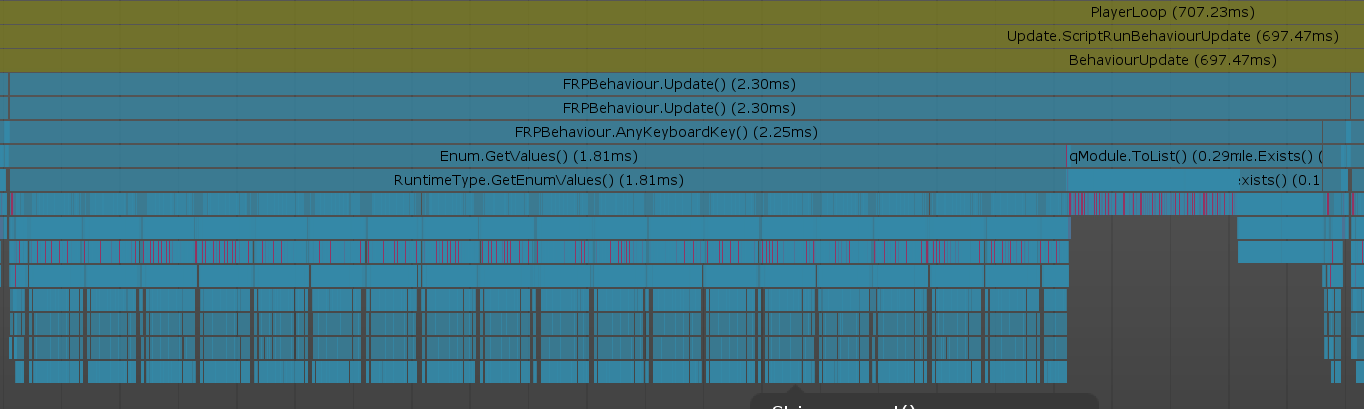
\includegraphics[width=\textwidth]{00-images/FRP-profiling.png}
    \caption{Distribution of execution time for a invocation of \ttt{Update} in a random frame in the Unit Management test with 250 units. Screenshot taken from Unity's Profiling Tool.}
    \label{fig:frp:profiling}
\end{figure}

\figref{frp:profiling} shows a screenshot of Unity's profiling tool after running it on the Unit Management scene with 250 units. This screenshot shows the distribution of execution time for a single frame. A total of 2.30 ms is spent in the \ttt{Update}-method of which 2.25 ms is used in the \ttt{FRPBehaviour.AnyKeyboardKey()}-method. This method is a part of the \gls{FRP}-system and iterates through all keyboard-keys to check if they are held down. This means that only 0.05 ms is spent executing code that updates the scene.

There are two problems with the strategy employed here:
\begin{enumerate}
    \item Each call to \ttt{FRPBehaviour.AnyKeyboardKey()} allocates a list of keyboard key ids with \ttt{Enum.GetValues()}, which takes 1.81ms.
    \item Each \ttt{FRPBehaviour} is actually a full-blown \gls{FRP}-system, which could very well be refactored into a singleton.
\end{enumerate}

The first problem is very simple to solve. We simply move the statement that alloces the list to a \ttt{static let}-field on the class, which ensures that a single list is shared among all instances of \ttt{FRPBehaviour}. This poses no problems as the list never assigned to.

The second problem requires a larger refactoring, as this relates to the Unity lifecycle of \ttt{GameObject}s. First and foremost some Unity methods are required to be tied to the \ttt{GameObject} they belong to. Examples of such methods are \ttt{OnCollisionEnter} and \ttt{OnTriggerExit}. Other methods, such as \ttt{Update} and reacting to keyboard strokes could, on the other hand, be tied to a \ttt{FRPEngine}. The problem here arises when \ttt{GameObject}s are destroyed. We have not added support to remove \ttt{FRPBehaviour}s from the \gls{FRP}-system, as the current version \dquote{cleans} up after itself when \ttt{GameObject}s are destroyed. This is to be understood in the sense that the whole system is deallocated and thus never risks invoking event handlers on objects that have been destroyed.

In order to truely determine whether or not \gls{FRP} comes with a performance penalty, these changes would have to be incorporated.
